\begin{figure}[H]
	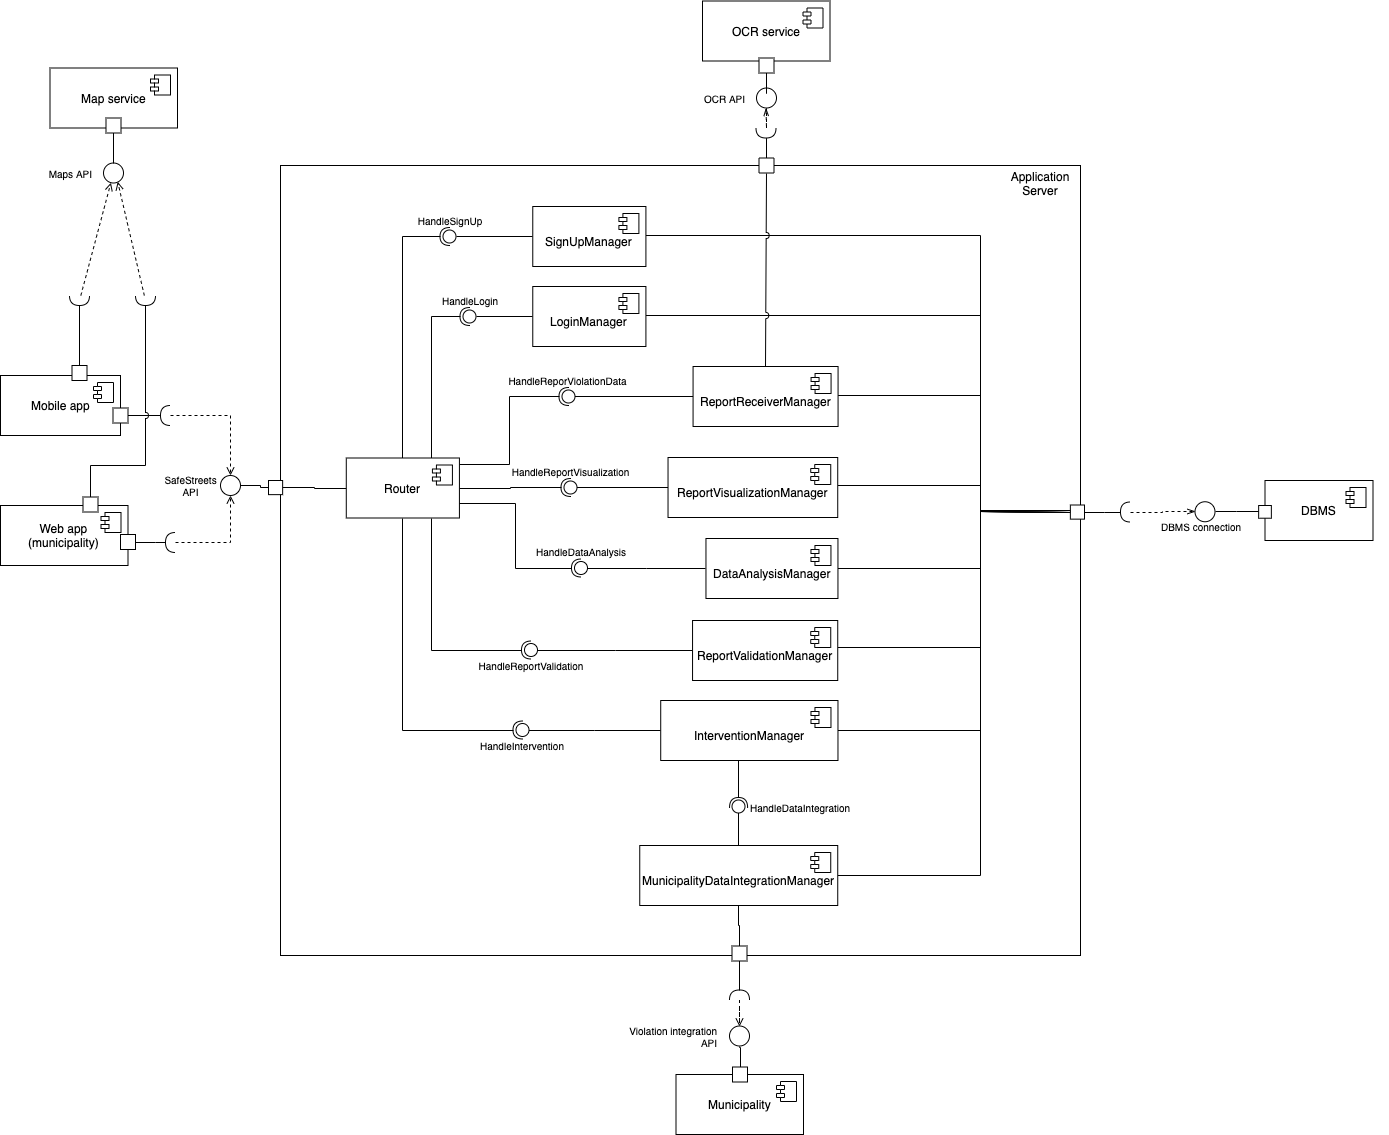
\includegraphics[width=\linewidth]{componentsDiagram.png}
\end{figure}
TODO: Change names of the interfaces and complete it

External interfaces:
\begin{itemize}
	\item DBMS
	\item Maps API
	\item OCR API
\end{itemize}

Customers app interfaces:
\begin{itemize}
	\item MobileApp (citizen/authorities)
	\item WebApp (municipality)
\end{itemize}

Internal services:
\begin{itemize}
	\item Router
	\item SignUpManager
	\item LoginManager
	\item ReportReceiverManager
	\item ReportVisualizationManager
	\item ReportValidationManager
	\item DataAnalysisManager
	\item InterventionManager
	\item MunicipalityDataIntegrationManager
\end{itemize}

\bigskip
Router:\\
Interfaces accessible from mobile app:
\begin{itemize}
	\item HandleSignUp
	\item HandleLogin
	\item HandleReportViolationData
	\item HandleReportVisualization
	\item HandleDataAnalysis
	\item HandleReportValidation
\end{itemize}
Interfaces accessible from municipality web app:
\begin{itemize}
	\item HandleSignUp
	\item HandleLogin
	\item HandleDataAnalysis
	\item HandleIntervention 
\end{itemize}

\bigskip
Component descriptions:
\begin{itemize}
	\item \textbf{Router:} 
	it listens for all requests made by clients on the SafeStreets API endpoints and provide handler for each type of request. Handlers defined by router call various managers internal to the application server that are pertinent to the request made by client, so that the router can receive from them the result of the operation and send back to the user a response.
	\item \textbf{SignUpManager:}
	module with the goal of handling registration requests of all user types. It checks that no data is missing and its correctness, by checking if the email is already been registered and if the password satisfy the given rules (ex. at least 8 characters, at least 1 number ecc...) and it's correctly repeated in the "repeat password" field. If data provided by the registration is valid, than the manager registers the account by inserting it into the main database and returns a confirmation to the router, else it returns an error.
	\item \textbf{LoginManager:}
	module that handles login requests made by clients. It checks that email and password provided by the user in the login form is actually associated to an account registered in the database. Returns a confirmation to router module if login is successful, otherwise it returns an error.
	\item \textbf{ReportReceiverManager:}
	module that allows the correct receipt of the reports data generated by the users and also the communication with the OCR service to recognize correctly the license plates. When a citizen start the report generation procedure, it will be asked to take pictures of the violations, in which is stated that the first one should have the license plate of the vehicle involved in the violation clearly visible. After the user takes the pictures, the first one is sent to the server and then is passed to this manager that then request the OCR service to recognize the license plate. After receiving the result, the manager forwards it to the router and it's sent back to the user for confirmation. The managers also handles the whole report data when the citizen submits it to the application server, completing it with some meta data like the timestamp and the user ID of the citizen, then it stores the report in the database.
	\item \textbf{ReportVisualizationManager:}
	module associated to single reports data requests or list of reports requests. It provide the possibility to query database for searching reports associated to a specific city or to a specific user, or a single report given its id. This covers all the functionalities regarding specific report visualization that the users can made with the mobile apps. In fact, authorities can access a list of all reports that are related to their city and a citizen instead can access the list of all reports made by himself; both type of users of users can then select a report from the lists and send a request to the router module with the report id attached. It's important that the ReportVisualizationManager checks what type of account made the request so that can check if the request is valid or it's fraudulent and avoid the possibility of not authorized data access. (TODO: SessionManager missing, better explicitly declare it (used by many managers, will complicate the diagram a lot)?)  
	\item \textbf{ReportValidationManager:}
	module that permits a report validation or invalidation made by authorities. It associates the authority ID to the report and changes the status of the report according to the one selected by the supervisor. Obviously the changes are made directly on the database, updating the record with the ID of the report present in the request.
	\item \textbf{DataAnalysisManager:}
	\item \textbf{InterventionManager:}
	module that handles municipalities' requests for generating new lists of possible interventions, targeted to provide possible solutions to the frequent violations in the most unsafe areas of their cities. Before generating the interventions, this module calls the MunicipalityDataIntegrationManager to integrate municipality data in the database, if possible. After receiving a response from the integration manager, the list of interventions will be generated. An algorithm consults all the reports present in SafeStreets database that are located in the city of the municipality that made the request, and checks for the areas with the highest density of violations. After computing the most unsafe areas of the city, the algorithm checks the type of violations recurring and from that it computes all possible interventions that can solve the problem. When all the process is finished, the result is returned to the router, in combination of a possible error raised from the MunicipalityDataIntegrationManager so that the user is aware of the fact that data integration was not possible and he could investigate the problem.
	\item \textbf{MunicipalityDataIntegrationManager:}
	module that allows the integration of violation data from any municipality API structured according to SafeStreets API. It is accessed by the InterventionGenerationManager when a municipality request the generation of a list of possible interventions to do in its territory. The module checks if the municipality that made the request has provided an API for accessing its data, if present in the database it requests all violation data that have a date later than the one indicated in last intervention generation timestamp (gets all data if no intervention generation was made by the municipality in the past), and integrate it in SafeStreets database. When the process is done the manager notifies the InterventionGenerationManager, that waits a response from it before initiating the intervention generation. Note that if no API is associated to municipality the integration will be immediately aborted, instead if the municipality's API endpoints or its provided data has not the structure expected the MunicipalityDataIntegrationManager will return an error to the InterventionGenerationManager, that will continue without the data integration using only data contained in SafeStreets database (the error is reported to the user in this case).
\end{itemize}